\section{Evaluación de negocio}
\label{sec:negocio_eval}

Esta sección traduce las métricas de la fase~4 a decisiones, siguiendo la fase~5
de CRISP-DM.

\subsection{El error de nivel no genera ahorro}

El error que importa en una operación de compra/venta es el MAE en Bs por USD
multiplicado por el monto operado. A una hora el ARIMA y el naïve empatan
(\textbf{0{,}0050}~Bs/USD) y a un día también (\textbf{0{,}0277}): \textbf{el
ahorro por precisión es cero a cualquier volumen}. La única diferencia medible
es el RMSE a una hora, $4{,}5$\,\% mejor, y no se traduce en ahorro porque el
MAE es idéntico.

\subsection{La señal direccional solo sirve a una hora}

Si el modelo se usa para decidir \emph{cuándo} comprar, lo que pesa es la
asimetría entre comprar y que baje (falso positivo) y no comprar y que suba
(falso negativo), no el error medio. Las matrices usan las predicciones de origen
móvil de la sección~4.4:

\begin{table}[!ht]
\centering\small
\begin{tabular}{@{}llcc@{}}
\toprule
Horizonte & & predice sube & predice baja \\
\midrule
1~h  & real sube & 45 (TP) & 29 (FN) \\
     & real baja & 31 (FP) & 35 (TN) \\
\addlinespace
24~h & real sube & 56 (TP) & 54 (FN) \\
     & real baja & 30 (FP) & 23 (TN) \\
\bottomrule
\end{tabular}
\caption{Matriz de confusión de dirección del nivel del blue (ARIMA con origen
móvil). Accuracy $0{,}571$ a 1~h ($n=140$) y $0{,}485$ a 24~h ($n=163$).}
\label{tab:matriz_costos}
\end{table}

A una hora el modelo evita 35 de las 66 bajadas y pierde 29 subas: conviene
mientras $35\,C_{FP} > 29\,C_{FN}$, es decir \textbf{siempre que
$C_{FN}/C_{FP} < 1{,}21$}. Con costos simétricos ahorra 6 de 66 unidades
($9{,}1\%$). A un día la relación se invierte y el umbral cae a
$23/54 = 0{,}43$, con accuracy por debajo del azar: \textbf{la señal direccional
es un fenómeno de una hora, no de un día}.

\begin{figure}[!ht]
\centering
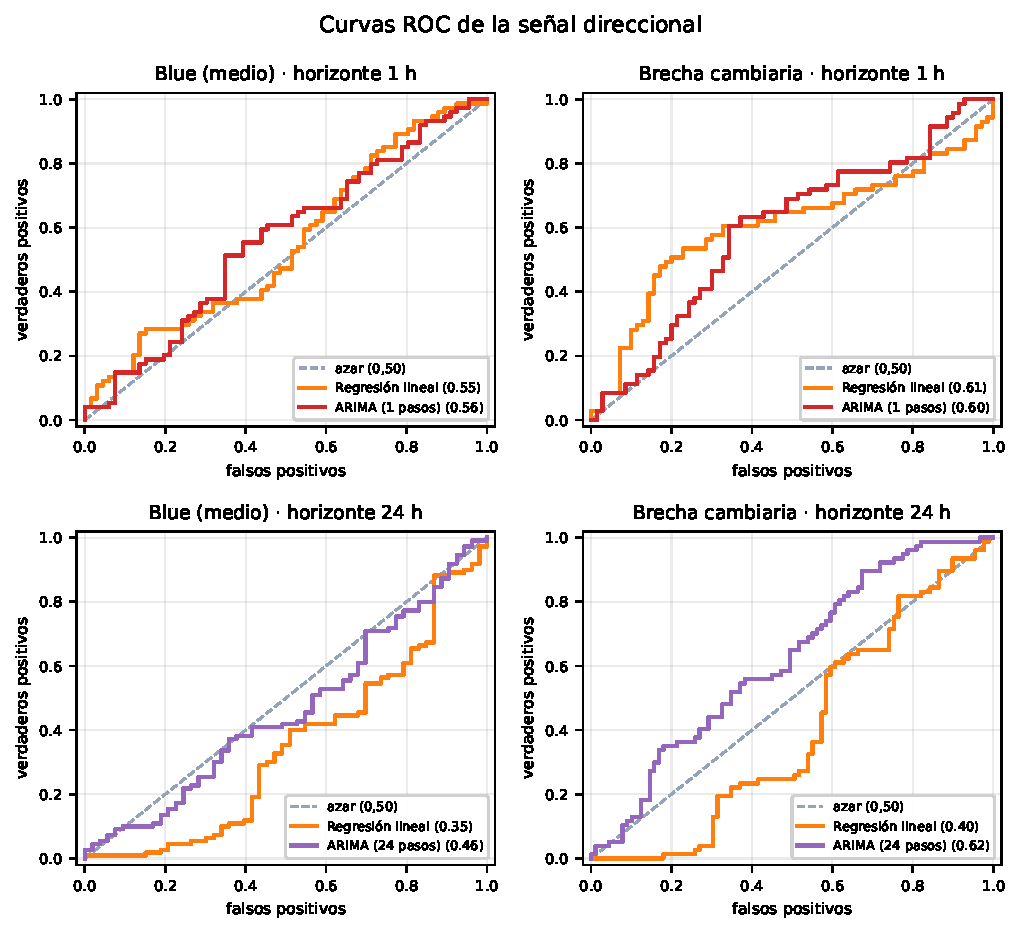
\includegraphics[width=\textwidth]{fig_roc.pdf}
\caption{Curvas ROC de la señal direccional, por horizonte (filas) y target
(columnas). La diagonal punteada es el azar (AUC $=0{,}50$). A una hora ninguna
curva pasa de $0{,}61$; a un día la brecha alcanza $0{,}62$ pero el nivel del
blue cae por debajo de $0{,}50$, y la regresión lineal queda en
$0{,}35$--$0{,}40$, peor que el azar.}
\label{fig:roc}
\end{figure}

\textbf{Lectura.} A una hora la discriminación es débil (AUC $0{,}55$--$0{,}61$),
coherente con un mercado casi impredecible. A un día la brecha mejora ($0{,}62$)
mientras el nivel cae bajo el azar, porque el sesgo de nivel de la regresión
invierte el signo de sus predicciones.

\subsection{Limitaciones de la evaluación}

\begin{itemize}
  \item El ahorro supone fijar el precio con el pronóstico; a precio de mercado
        es cero.
  \item $C_{FP}$ y $C_{FN}$ no se estimaron con datos de la empresa: el
        resultado es un umbral de decisión, no una cifra contable.
  \item Una sola semana de evaluación: los umbrales deben revisarse con más
        ventanas antes de usarse operativamente.
\end{itemize}
